\documentclass[12pt,a4paper,BCOR12mm, headexclude, footexclude, twoside, openright]{scrartcl}
\usepackage[scaled]{helvet}
\usepackage[british]{babel}
\usepackage[utf8]{inputenc}
\usepackage[T1]{fontenc}
\usepackage{fancyhdr}
\usepackage{lastpage}
\usepackage{ifthen}
\usepackage{amsmath,amsfonts,amsthm}
\usepackage{sfmath}
\usepackage{makecell}
\usepackage{booktabs}
\usepackage{sectsty}
\usepackage{xcolor}
\usepackage{tikz}
\usepackage{hyperref}
%\KOMAoptions{optionenliste}
%\KOMAoptions{Option}{Werteliste}

\newcommand*{\TakeFourierOrnament}[1]{{%
\fontencoding{U}\fontfamily{futs}\selectfont\char#1}}
\newcommand*{\danger}{\TakeFourierOrnament{66}}
\addtokomafont{caption}{\small}
%\setkomafont{descriptionlabel}{\normalfont
%	\bfseries}
\setkomafont{captionlabel}{\normalfont
	\bfseries}
\let\oldtabular\tabular
\renewcommand{\tabular}{\sffamily\oldtabular}
\KOMAoptions{abstract=true}
%\setkomafont{footnote}{\sffamily}
%\KOMAoptions{twoside=true}
%\KOMAoptions{headsepline=true}
%\KOMAoptions{footsepline=true}
\renewcommand\familydefault{\sfdefault}
\renewcommand{\arraystretch}{1.1}
\newcommand{\horrule}[1]{\rule{\linewidth}{#1}}
\setlength{\textheight}{230mm}
\allsectionsfont{\centering \normalfont\scshape}
\let\tmp\oddsidemargin
\let\oddsidemargin\evensidemargin
\let\evensidemargin\tmp
\reversemarginpar

\numberwithin{equation}{section} % Number equations within sections (i.e. 1.1, 1.2, 2.1, 2.2 instead of 1, 2, 3, 4)
\numberwithin{figure}{section} % Number figures within sections (i.e. 1.1, 1.2, 2.1, 2.2 instead of 1, 2, 3, 4)
\numberwithin{table}{section} % Number tables within sections (i.e. 1.1, 1.2, 2.1, 2.2 instead of 1, 2, 3, 4)

\setlength\parindent{0pt}

\definecolor{C000000}{HTML}{000000}
\definecolor{CFFFFFF}{HTML}{FFFFFF}
\definecolor{C00FF00}{HTML}{00FF00}
\begin{document}
%\sffamily
\fancypagestyle{plain}
{%
  \renewcommand{\headrulewidth}{0pt}%
  \renewcommand{\footrulewidth}{0.5pt}
  \fancyhf{}%
  \fancyfoot[R]{\emph{\footnotesize Page \thepage\ of \pageref{LastPage}}}%
  \fancyfoot[C]{\emph{\footnotesize Samy Aittahar}}%
}

\thispagestyle{plain}

\titlehead
{
	University of Liège\hfill
    INFO8006%
}

\subject{\vspace{-1.0ex} \horrule{2pt}\\[0.15cm] {\textsc{\texttt{Introduction to AI}}}}
\title{Project: Pac Man \\}
\subtitle{\textsc{\texttt{Thanks to Berkeley University}}\\\horrule{2pt}\\[0.5cm]}
\author{\bfseries{Samy Aittahar}}
\date{}

\maketitle

\vspace{-1.5cm}

%--------------------------------------------

\section{Pratical Information}
\begin{itemize}

    \item Deadline: December 22.
    \item You must work in {\bf groups of 2 students}.
    \item Deliverable 1: A Python implementation of the classes \texttt{Agentsearch} and \texttt{Agentghost}, as defined in the  \texttt{agentsearch.py} and \texttt{agentghost.py} templates. See source code for more details.
    \begin{itemize}
    	\item \danger If your agent's action violates the game constraints, it will be ignored.
        \item You are free to use any library, as long as it does not hurt your code organization and clarity, and you are able to explain the principles behind it.
        \item The name of your agent classes should be \texttt{Agentsearch\emph{numstudent1}\emph{numstudent2}} and \texttt{Agentghost\emph{numstudent1}\emph{numstudent2}} where \emph{numstudent1} and \emph{numstudent2} are your student IDs without the "s". The names of your main agent class file should be respectively \texttt{agentsearch\emph{numstudent1}\emph{numstudent2}.py} and \texttt{agentghost\emph{numstudent1}\emph{numstudent2}.py}.
    \end{itemize}
    \item Deliverable 2: A report of 7 pages max. in which should appear, for each stage of the project:
    	\begin{itemize}
        	\item The approaches you have considered to implement your agents.
            \item Their limitations for the current and the next stage of the project.
            \item Comparisons with some naive approaches.
            \item Briefly but clearly discuss about better strategies than your current work. "We could use X" is not enough, you need to explain the benefits (and drawbacks) of the claimed "better" approaches.
        \end{itemize}
    \item Upload your deliverables as a tar.gz archive on the \href{http://submit.montefiore.ulg.ac.be/student/viewprojects/INFO8006}{Montefiore submission platform}.

	\item You will be evaluated on the following criteria:
    \begin{itemize}
		\item Score and computation time of your agents.
        \item Organization and clarity of your code.
        \item Quality of your report.
	\end{itemize}
\end{itemize}

\section{Pac-Man Game}

The games consists in eating all food dots while avoiding ghosts in a fully observable maze. The game ends when either Pacman has eaten all the food dots (winning game) or has been hit by a ghost (game over). Figure \ref{fullmaze} shows an example of a Pacman maze with a single food dot.

\subsection{Step 1 : Search}

Pacman is let alone in a maze with an arbitrarily distribution of food dots over the map. The goal is to eat them all while minimizing a score based on the time spent to eat the food dots.\\

You are encouraged to try several algorithms as described in the \emph{Search} lecture. Remember there is an implicit time limit, as the game engine does not wait your computation to go on.

Implement the \texttt{Agentsearch} class template to address this step. More details can be found in the source code.

\begin{figure}
	\label{fullmaze}
	\begin{center}

	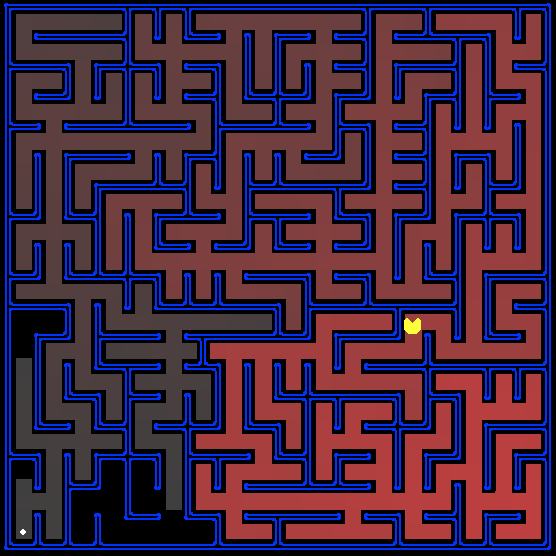
\includegraphics[scale=0.5]{pacmazefull.png}
    \caption{Pac man and food dots in a maze}
    \end{center}
\end{figure}





\subsection{Step 2 : Search + Ghosts}

Ghosts (one or more) are added to the maze. Pacman must avoid them while
collecting the food dots. If Pacman collides with a ghost, the game ends there
with a negative score. All ghost agents will behave using one of the following
policies:

\begin{itemize}
	\item Pattern 0: Counterclockwise left (see Figure \ref{counterclockwise} for more details).
    \item Pattern 1: Always move greedily towards Pacman or flee greedily from Pacman in eater mode.
    \item Pattern 2: Semi-random pattern. The next action is taken using the following strategy:
    \begin{itemize}
    	\item Follow pattern 1 with 50\% probability.
        \item Follow pattern 0 with 25\% probability.
        \item Pick a random valid move with 25\% probabiliy.
    \end{itemize}
    \item Pattern 3: either pattern 0, 1 or 2, but which of those policies is used by the ghost is unknown to Pacman.
\end{itemize}

\begin{figure}
	\label{counterclockwise}
	\begin{center}

	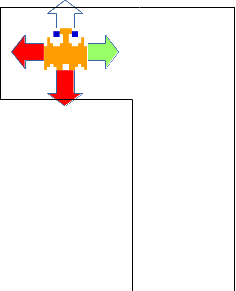
\includegraphics[scale=1]{ghostclockwiseleft.png}
    \caption{Counterclockwise left. Ghost try first to go left and if it is not possible, analyze moves in a counterclockwise order until a legal move is found}
    \end{center}
\end{figure}

Capsules are also added to the game. When Pacman eats a capsule, he gains the ability to eat the ghosts for a fixed amount of time, which will be provided to the Agentghost class. An eaten ghost reappears immediately in its initial position.\\

Like in the previous step, you are encouraged to compare several approaches described in lectures or even coming from other sources. In the latter case, you'll have to explain carefully the principles behind the chosen approaches.

Implement the \texttt{Agentghost} class template to address this step. More details can be found in the source code.


\end{document}
